\section{Product Perspective}
The \emph{Travlendar+} Software has as main goal to schedule all the user's appointments in a comfortable and useful way: planning the optimal travel solution to allow the user to reach his appointments in time.

To do that, the user has to give his tasks to our System, then the System creates a possible calendar considering user's preferences, tasks' priorities and roads status; asking directly to the user in case of conflicts.

The various trips between tasks may rely on public transport, in that case the System will suggest the user the best ticket option, trying to minimize the user expense considering the whole calendar's appointments. Otherwise, if is it the case of a shared based travel mean, the System will allow the user to book and later rent such vehicle through the appropriate site or application.
Since it is unrealistic to guarantee a precise schedule when accounting for shared-based travel means, due to a series of problems out of the scope of the application\footnote{When the \emph{Travlendar+} application has to schedule a trip with a shared based travel mean it cannot be sure that a shared-based vehicle will be available in that zone at that time}, the System will check the availability of the vehicle before the trip starts and later notify the user, suggesting a reservation time for a close vehicle or another travel option.    

The System provides a series of preferences settings, among the more relevant there are: the possibility to specify a repetition during the week of a certain task (also month-periodic or with user-defined periodic tasks) within a fixed, flexible or variable time slot; the possibility to define a maximum range for walking to reach a certain location; the possibility to avoid or prefer a certain travel mean, given the user vehicles' (eco-profile) or the time; finally a special task to reserve some breaks time to the user.

In addition, the user will be able to dynamically modify tasks' preferences and features, with different granularity options, receiving a new calendar schedule back.

\begin{figure}[H]
    \centering
    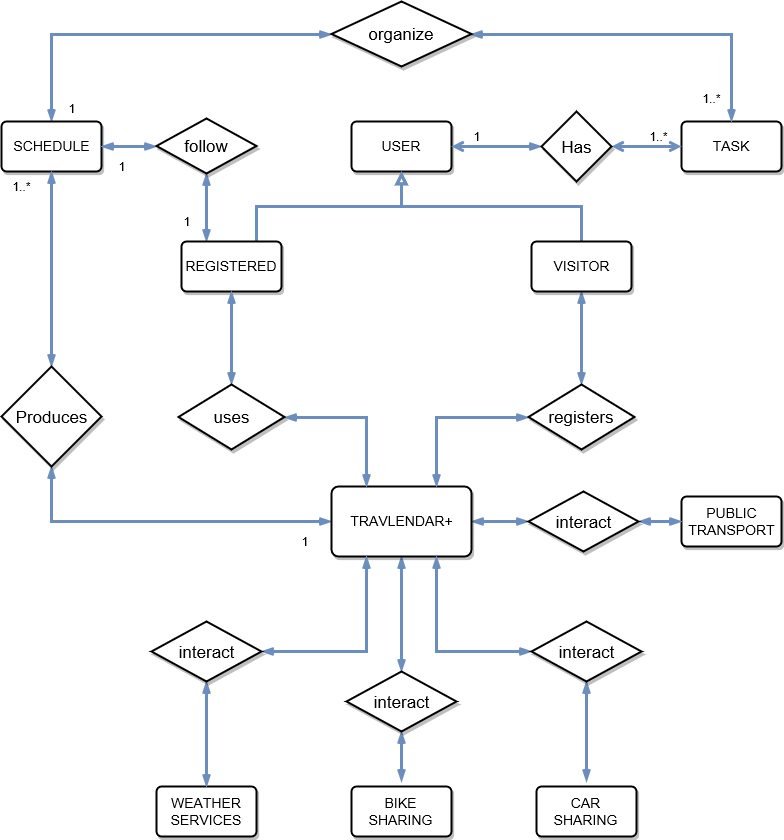
\includegraphics[scale=0.5]{Pictures/ScenarioER.png}
    \caption{ER Diagram of the \emph{Travlendar+} System}
\end{figure}
